\documentclass{article}
\usepackage[utf8]{inputenc}
\usepackage{graphicx}
\graphicspath{ {images/} }
\usepackage{listings}
\usepackage{color}
\usepackage{textcomp}
\usepackage{multicol}
\usepackage{float}

\title{CMPE460 Project 1 Report}
\author{
  Yiğit Özkavcı \\
  \texttt{2013400111} \\
  \texttt{yigit.ozkavci@boun.edu.tr}
}
\date{February 2018}

\begin{document}

\maketitle

\tableofcontents

\section{Introduction}
In this assignment, we are expected to write a ray tracer with ambient illumination targeting sphere objects.

It's a simple iteration on a 2d plane pixel by pixel to know what color each pixel corresponds to.

In the following sections, we will describe the method used without getting into implementation details (Section \ref{method}) and then we will describe how this problem is modeled in our c++ program(Section \ref{modeling}), and lastly talk about implementation of the problem(Section \ref{implementation}).

\section{Method}
\label{method}
\par As the ray tracing algorithm suggests, we first traverse through the plane pixels one by one. For each of these pixels, we invoke a $shoot_ray$ function, which given a vector and a list of spheres, returns a color. Indeed, it's signature is pretty self explanatory: it assigns a color to every pixel of the plane, being parametrized by the ray vector and all of the spheres available.

There are few issues to consider while sending the ray;
\par Firstly, when we run the intersection function on a ray and a sphere and we get a result, we need to make sure the resulting $t$ value is non-negative, that is the solution is found ``in front of the ray''. This is important because we can accidentally think that there is an obstricle when there really is not.

\par Another issue is that we need to deal with multiple intersections of the rays with spheres. We need to pick the closest intersection point, and this involves sorting the list of intersections. This method will further discussed in section \ref{complexity}.

\subsection{Complexity Analysis}
\label{complexity}
For simplicity, we collect all the intersection points and sort them afterwards in our implementation, but in an ideal world this would involve keeping the closest distance and conditionally set the closest one like finding a maximum number iteratively in a list.

Let's say the number of spheres is $S$ and the number of intersection points for a point in plane is $l$. Then the complexity of finding intersections then sorting is $O(S + l(logl))$.

There is a better way, though. We can keep a value for the distance between our point in plane and the \textbf{closest} intersection point, and if a found intersection point's distance is lesser than the value we keep, we update the \textbf{chosen} intersection point;

But\ldots unfortunately this does not work for our problem. Because when we are shadowing, we start looking for an intersection from a point \textbf{on} the sphere, and this makes the closest intersection point to be itself. So we are looking for the second closest point, which is also not always the case because of the floating point approximation. Hence, we use a parameter to calibrate this behavior by tolerating this $CLOSENESS$ property (see section \ref{tolerance} for more details)

\section{Tolerance}
\label{tolerance}
Consider these two points:

(201, 185, 90)
(201, 184, 90)

While looking for an intersection starting from the position on the sphere, if we get this result, this intersection is probably the same intersection point we just started out with.

In order to eliminate these cases, we measure the length, and if it's smaller than our constant value $CLOSENESS\_TOLERANCE$ we say they are the same points.

Indeed this yields a smoother output since it reduces the amount of errorneus points.

\section{Modeling}
\label{modeling}
In order to represent all those concepts we have in real life such as $ray$, $vector$, $position$, $sphere$, $plane$; we used abstractions in our C++ codebase.

These abstractions make our functions more readable and easy to work on. For instance, we have a function with the following signature:

\begin{lstlisting}[frame=single]  % Start your code-block

vector<intersection_t> *ray_sphere_intersection(
  vector_t ray_vec,
  vector<Sphere> spheres
);
\end{lstlisting}

Because of the proper usage of abstraction, we can only be interested in high-level objects and structs and focus on the real problem.

\section{Implementation}
\label{implementation}
The first thing our program does is to read the user input. It's being done by the read\_spheres() function. Input is read one by one, meaning in order to read a RGB value, we ask for each one of them one by one.

\par After getting all the information on spheres, we initialize our 2d plane, which is only a color\_t** for us. After we allocate the necessary 2d plane, we start shooting rays on it and modifying the plane data.

\par Shooting rays are done by the shoot\_ray function. It returns a color that it decided by shooting the mentioned ray, and we save the color into our 2d array.

After shooting for the pixel, we also check for the shadowing. We simple call the function shadow\_point() with parameters closest\_interaction and spheres. This function takes care of whether to desaturate that color or not based on that point's interaction with the spheres between it and the light source.

\subsection{Rendering}
\label{rendering}
In order to render our plane into an image, we used an open-source cpp library called bitmapimage \cite{bitmapimage}. We simply use this library to encode our color information in each pixel and set pixels. Indeed, we only use the image(), set\_pixel() and save\_image() functions from this library.

\newpage

\subsection{Examples}
\label{examples}
In all the examples, the light's position is (500, 500, 500) as the project document suggests.

\begin{centering}
\begin{figure}[H]
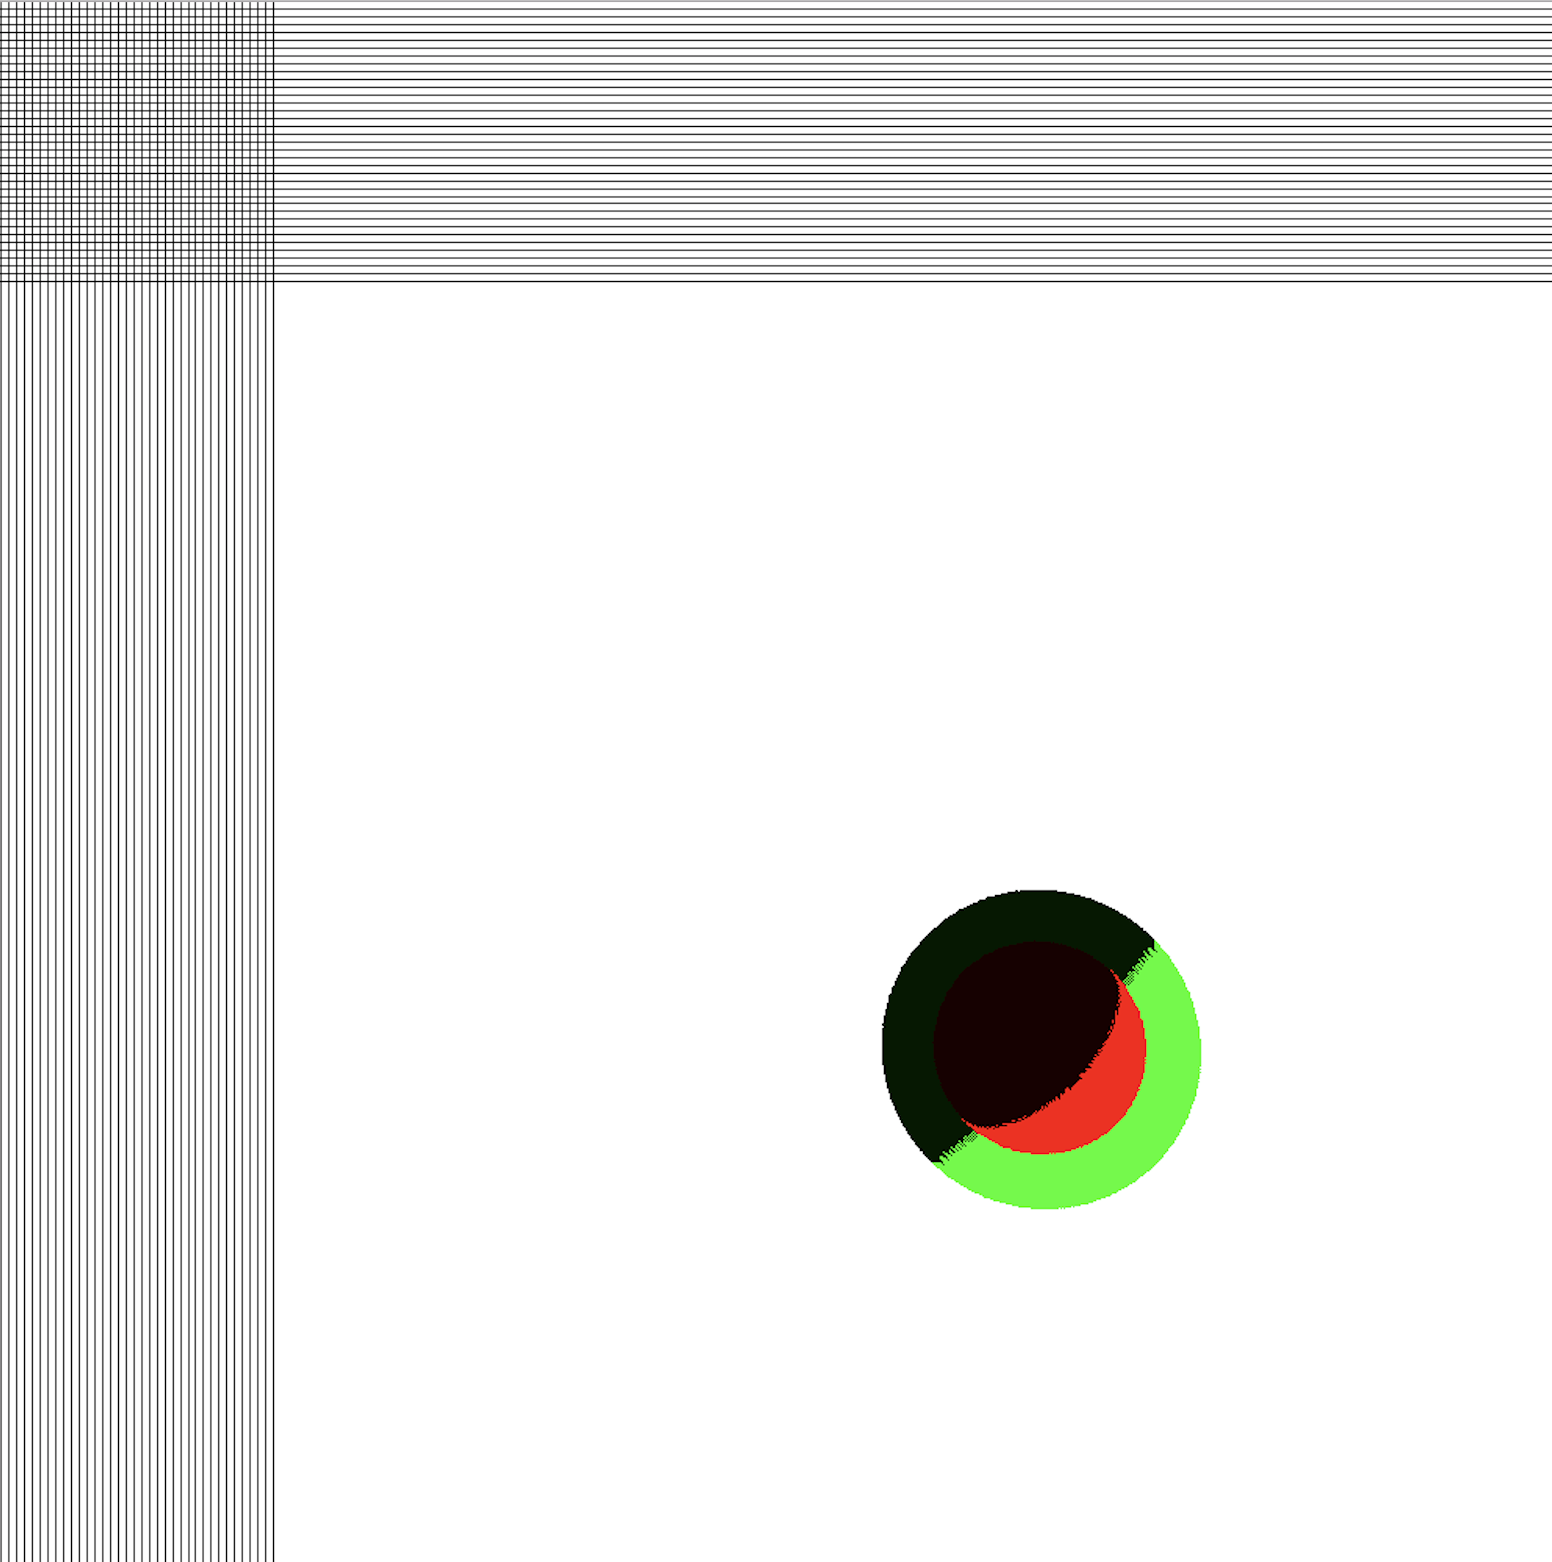
\includegraphics[width=1\textwidth]{./images/TestData.png}
\caption{With Test Data Described In Project Doc}
\label{fig:figure2}
\end{figure}
\begin{figure}[H]
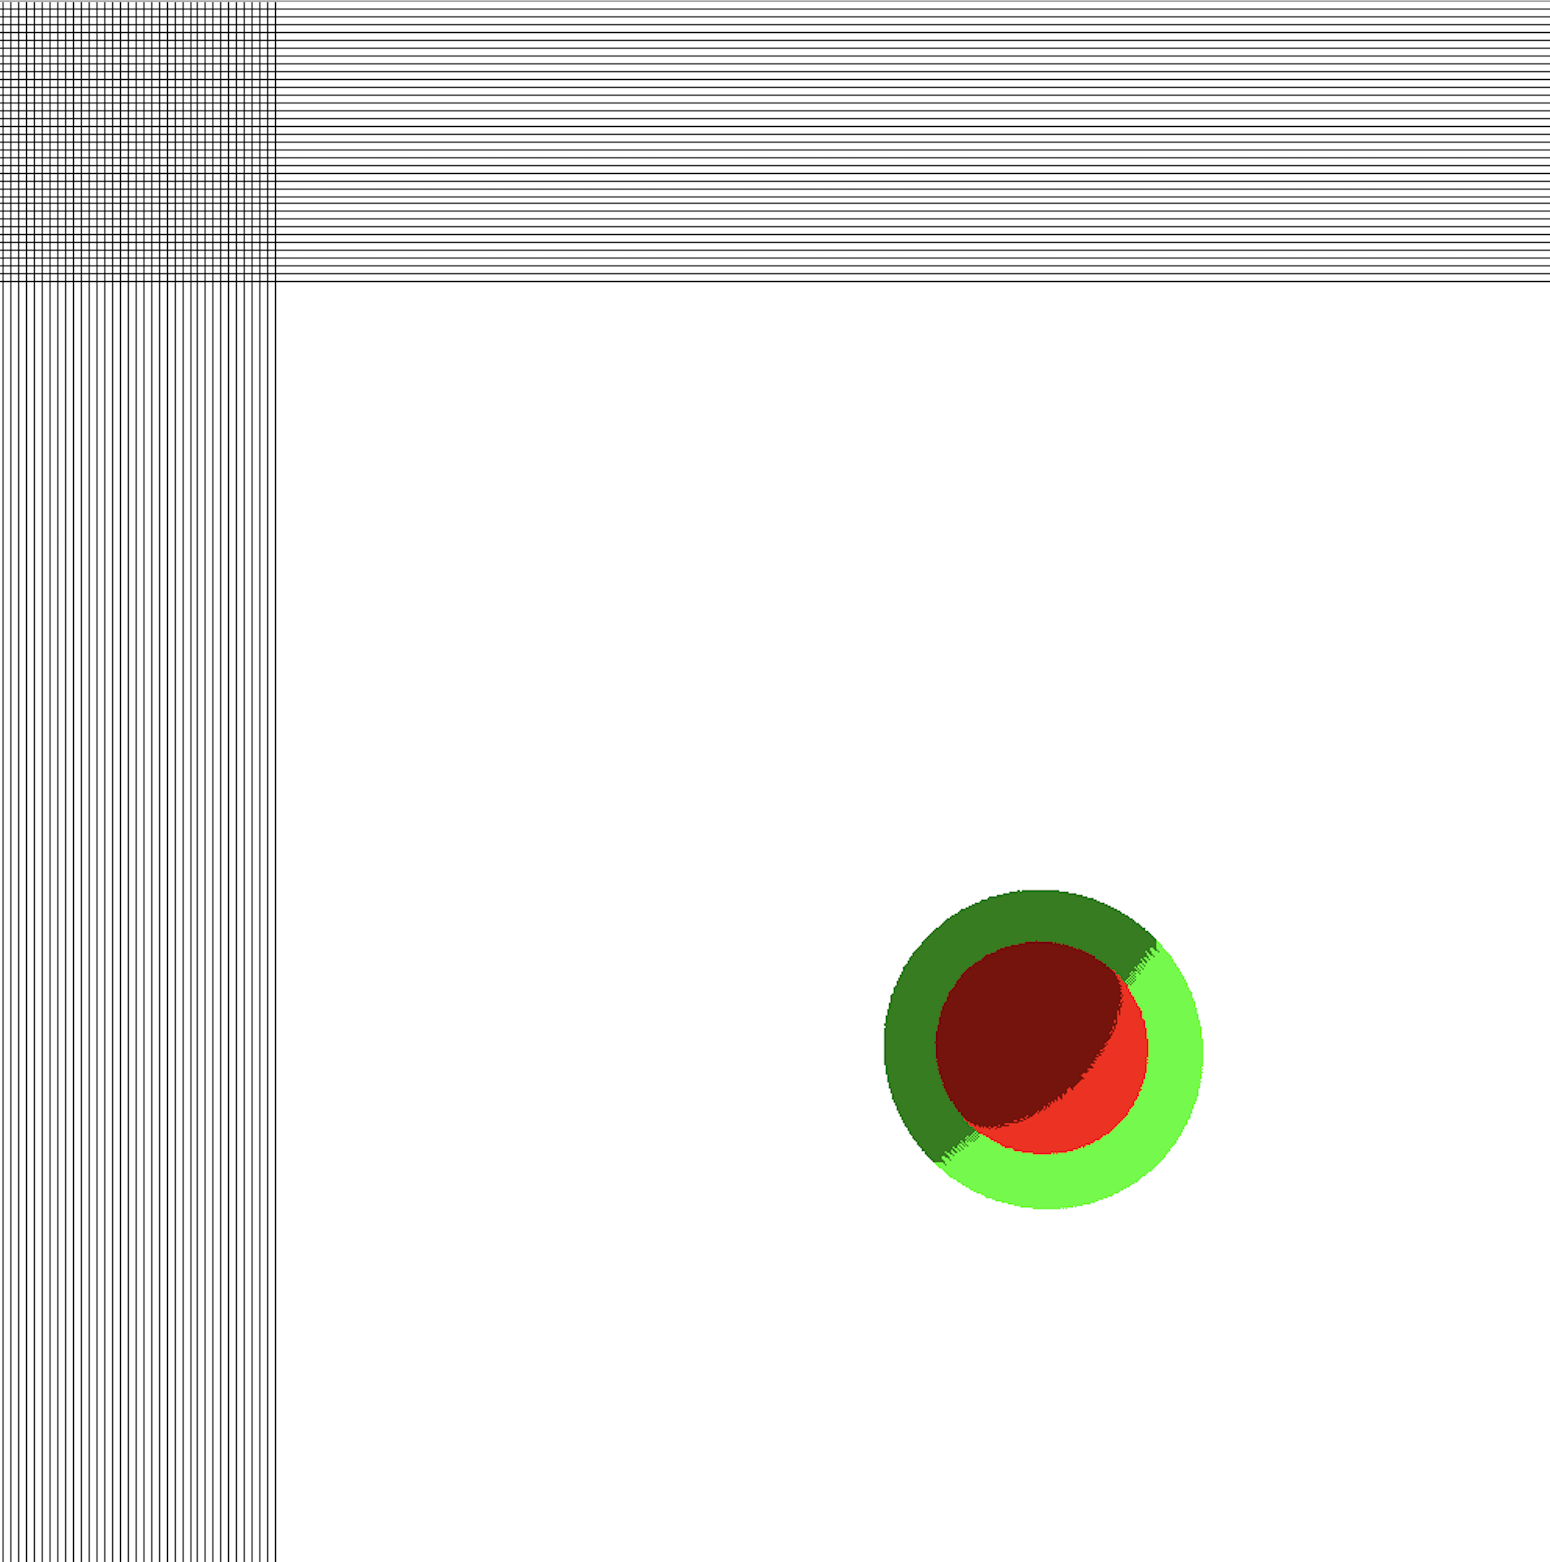
\includegraphics[width=1\textwidth]{./images/Ambient05.png}
\caption{With Ambient Light Coefficient Increased to 0.5}
\label{fig:figure2}
\end{figure}
\begin{figure}[H]
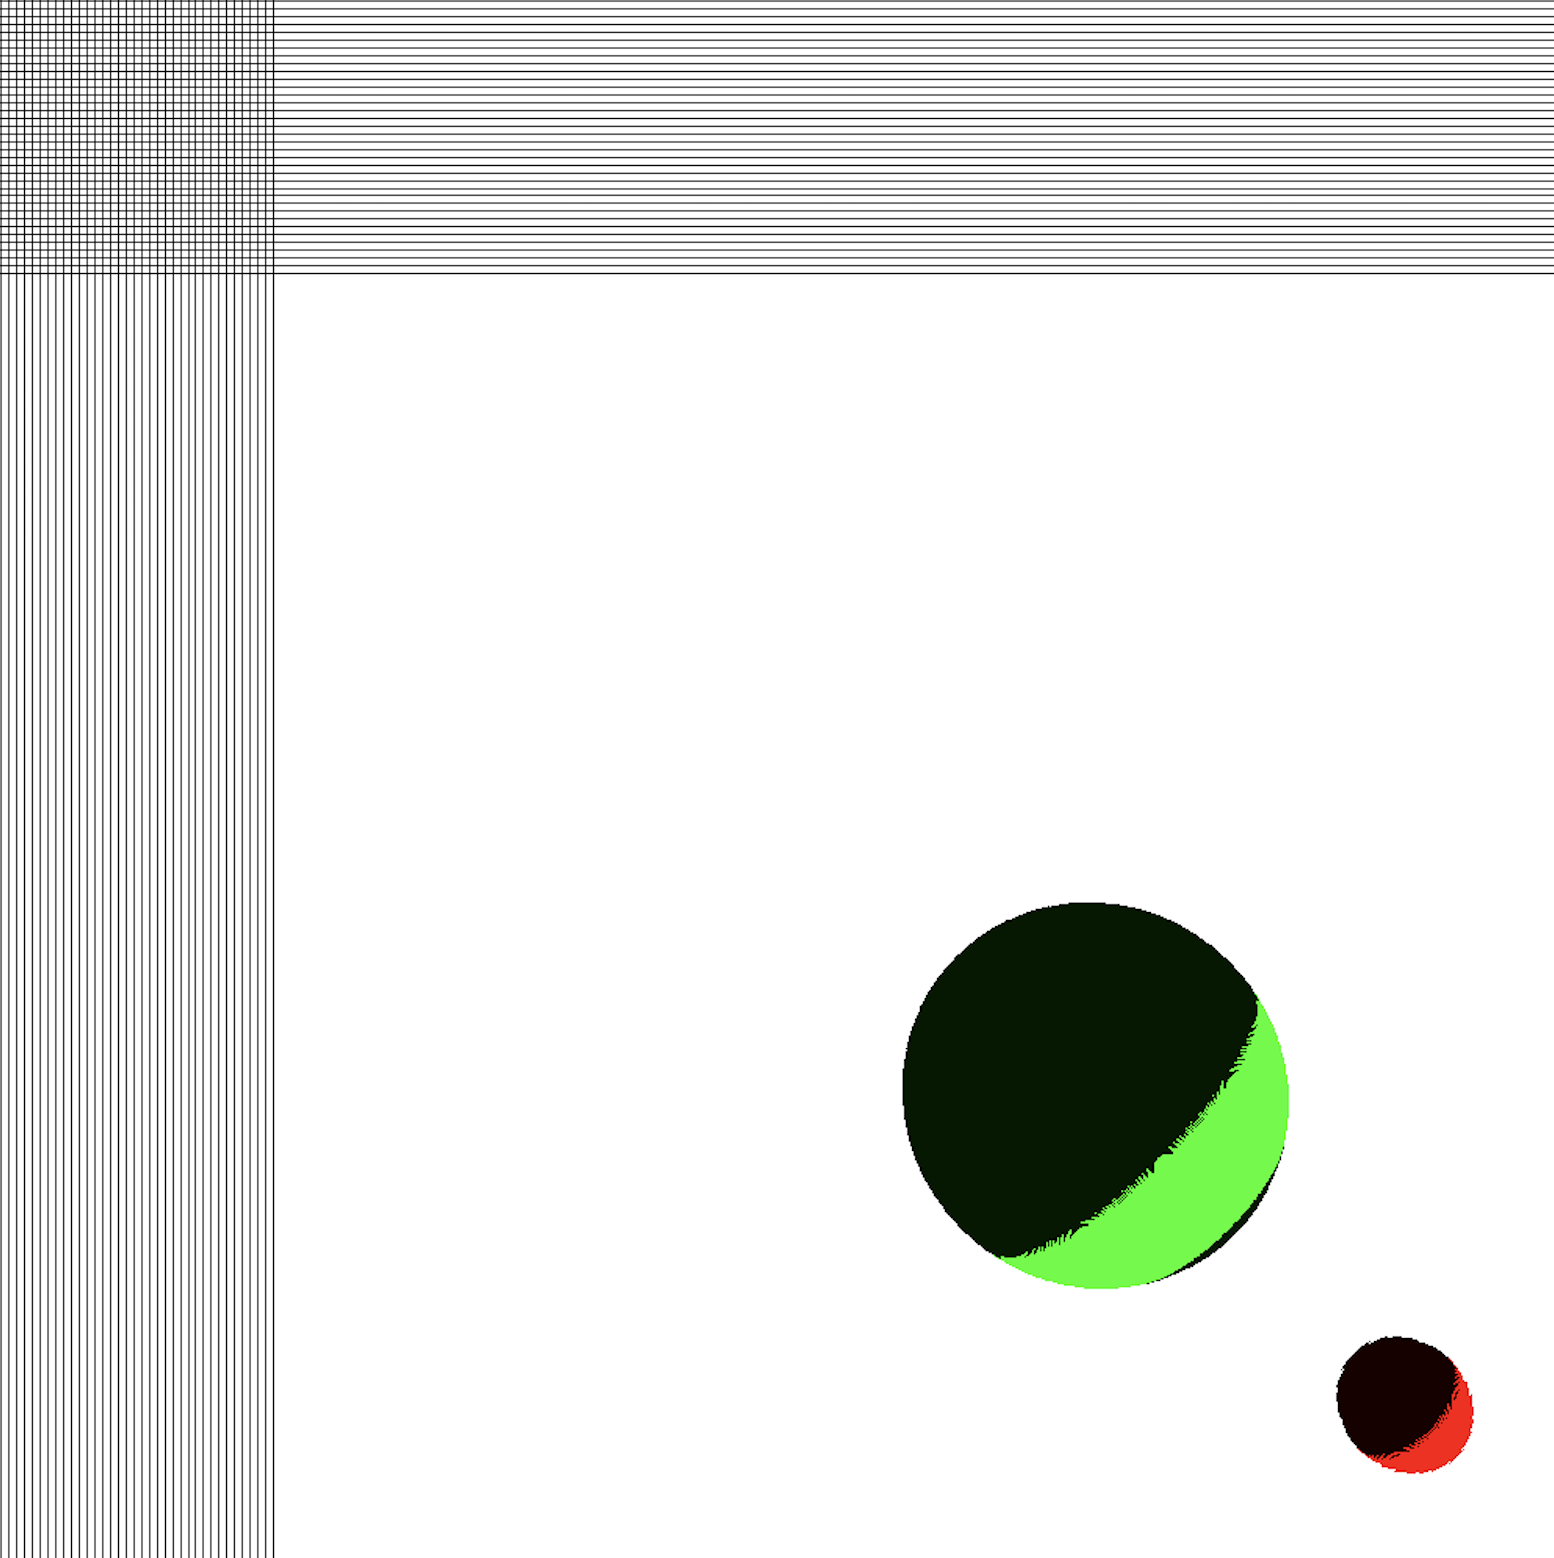
\includegraphics[width=1\textwidth]{./images/CloserLight.png}
\caption{With Light Being In Position (280, 280, 500) and Spheres Distinct}
\label{fig:figure2}
\end{figure}
\begin{figure}[H]
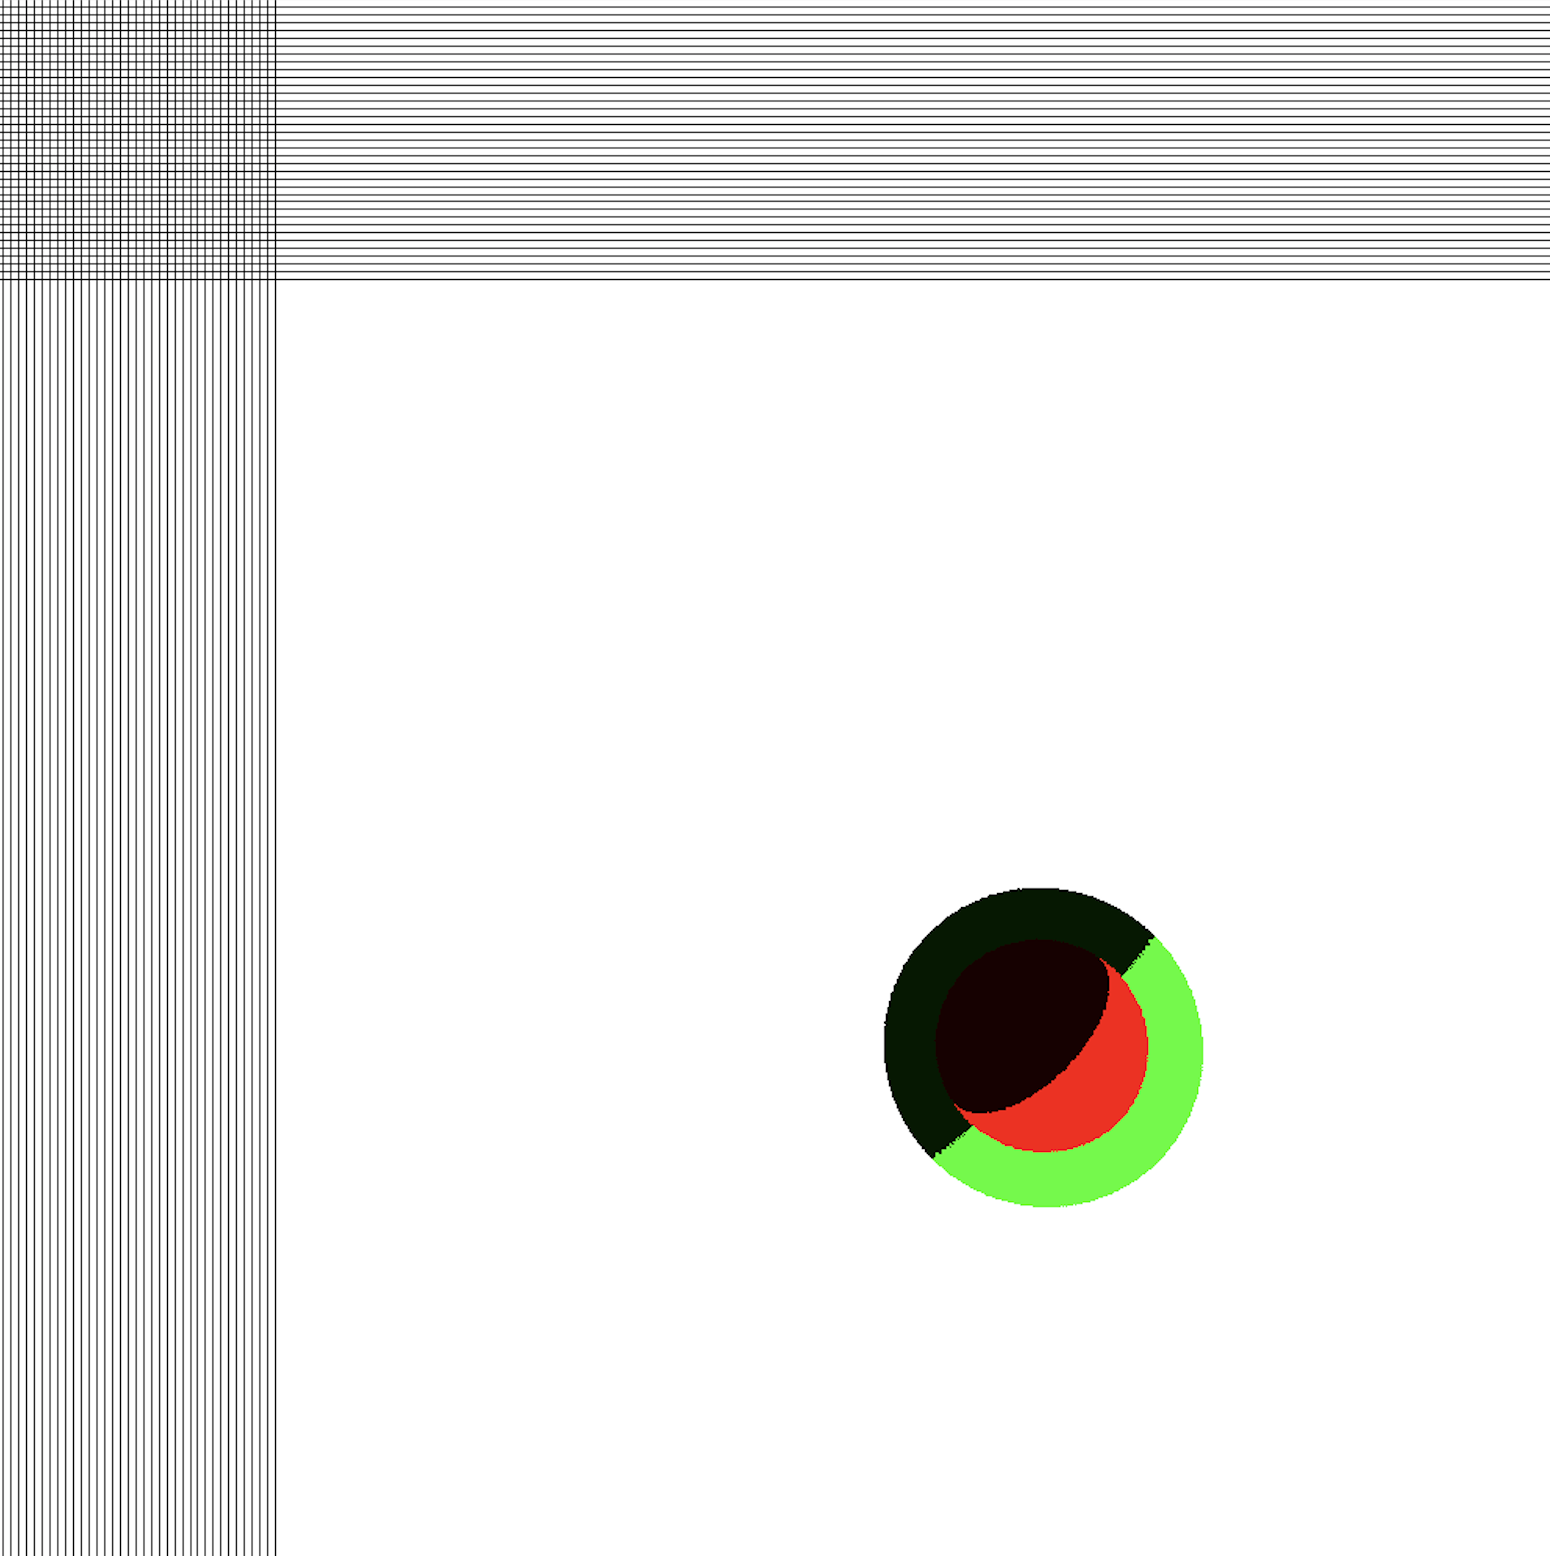
\includegraphics[width=1\textwidth]{./images/IncreasedTolerance.png}
\caption{With Increased CLOSENESS\_TOLERANCE}
\label{fig:figure2}
\end{figure}
\end{centering}

\begin{thebibliography}{9}
\bibitem{bitmapimage}
  https://github.com/ArashPartow/bitmap
\end{thebibliography}

\end{document}
